\chapter{RESULTADOS OBTIDOS}
\label{chp:resultadosObtidos}
 
Neste capítulo, serão apresentados os resultados que foram obtidos através da
ferramenta analítica \acs{Google Analytics} e as principais telas do sistema
web proposto por este projeto. Sendo que, os dados estatísticos apresentados
correspondem ao período de 11 de outubro à 09 de novembro de 2014.

Pode-se observar na Figura \ref{fig:googleAnalyticsGrafico}, que a
ferramenta de gestão de perguntas e respostas está sendo acessada quase
que diariamente para gerir as questões postadas na lista de discussão.

\begin{figure}[h!tb]
	\caption{Visualizações de página}
	\label{fig:googleAnalyticsGrafico}

	\centering
	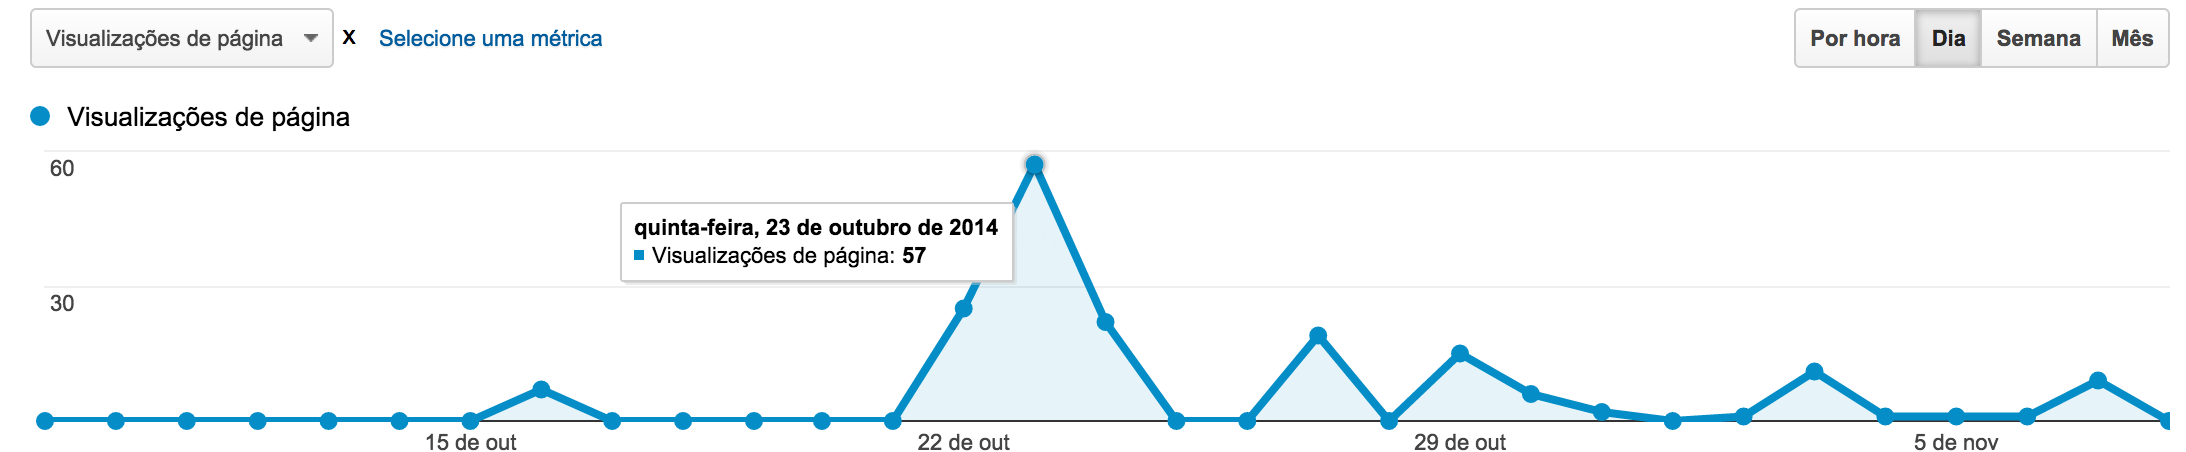
\includegraphics[width=\textwidth]{images/resultados/google-analytics-grafico.png}

	\centering
	\footnotesize Fonte: \fonteOAutor
\end{figure}

\FloatBarrier 	% Este comando impede que as imagens
				% flutuem a partir deste ponto no seu documento

Na data em que a ferramenta foi divulgada ao grupo ``Rumo à certificação PHP''
(no dia 23 de outubro de 2014), conforme exibe-se na Figura
\ref{fig:googleAnalyticsGrafico}, o número de visualizações de página atingiu 
57 \textit{page views}, enquanto que, o autor esperava que o número atingisse
apenas 30 visualizações. Ainda referente a data em que houve a divulgação, 
percebe-se que o tempo de acesso ao sistema também foi bastante elevado, sendo
que o tempo médio para esta única data atingiu 25:04 minutos conforme ilustra a 
Figura \ref{fig:googleAnalyticsTempoAcessoDivulgacao}.

\begin{figure}[h!tb]
	\caption{Tempo de acesso ao sistema no dia da divulgação da ferramenta}
	\label{fig:googleAnalyticsTempoAcessoDivulgacao}

	\centering
	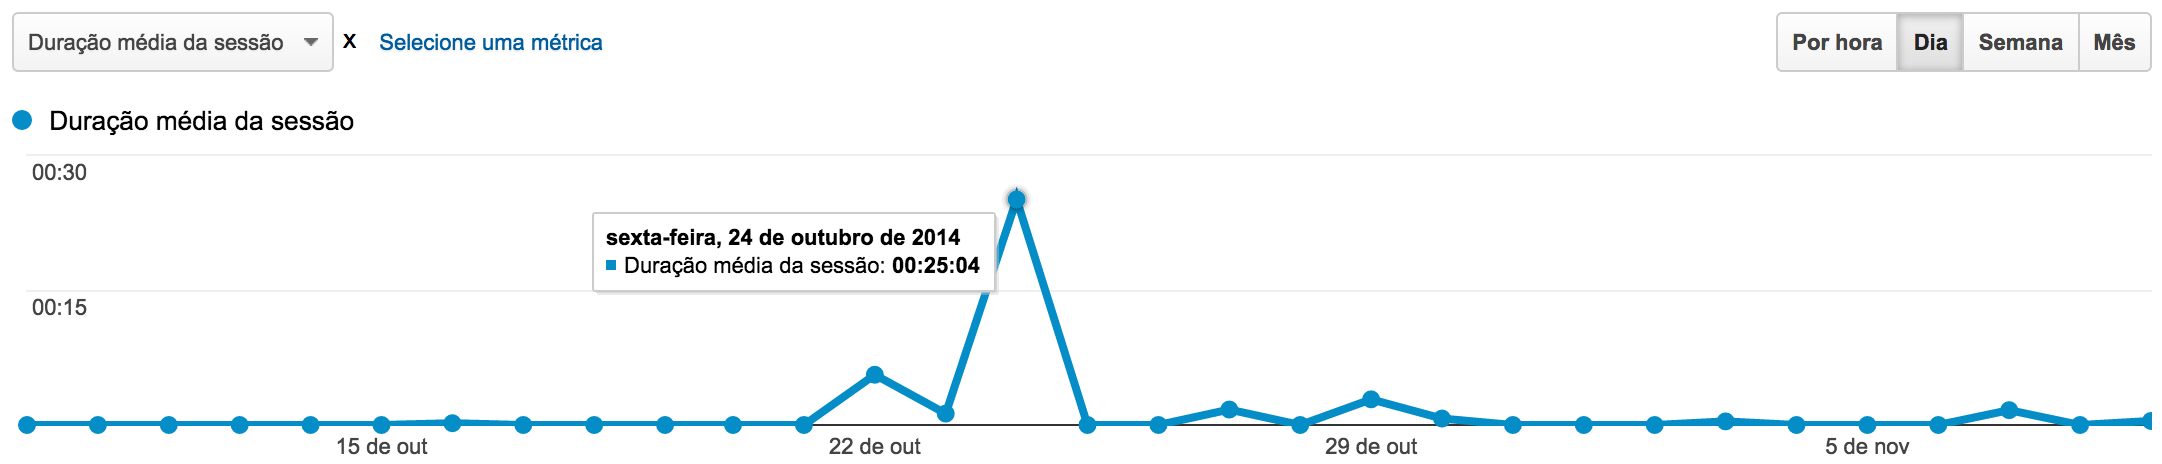
\includegraphics[width=\textwidth]{images/resultados/google-analytics-tempoacesso-divulgacao.png}

	\centering
	\footnotesize Fonte: \fonteOAutor
\end{figure}

\FloatBarrier 	% Este comando impede que as imagens
				% flutuem a partir deste ponto no seu documento
				
Nota-se também que nos dias seguintes a quantidade de visualizações de página
se estabilizou, onde removendo a data de divulgação da contagem a fim de não
influenciar no resultado final da média, foi obtido o valor de 25,40 acessos
semanais conforme os dados apresentados na Figura \ref{fig:googleAnalyticsMediaVisualizacoes}.

\begin{figure}[h!tb]
	\caption{Quantidade de visualizações de página semanais}
	\label{fig:googleAnalyticsMediaVisualizacoes}

	\centering
	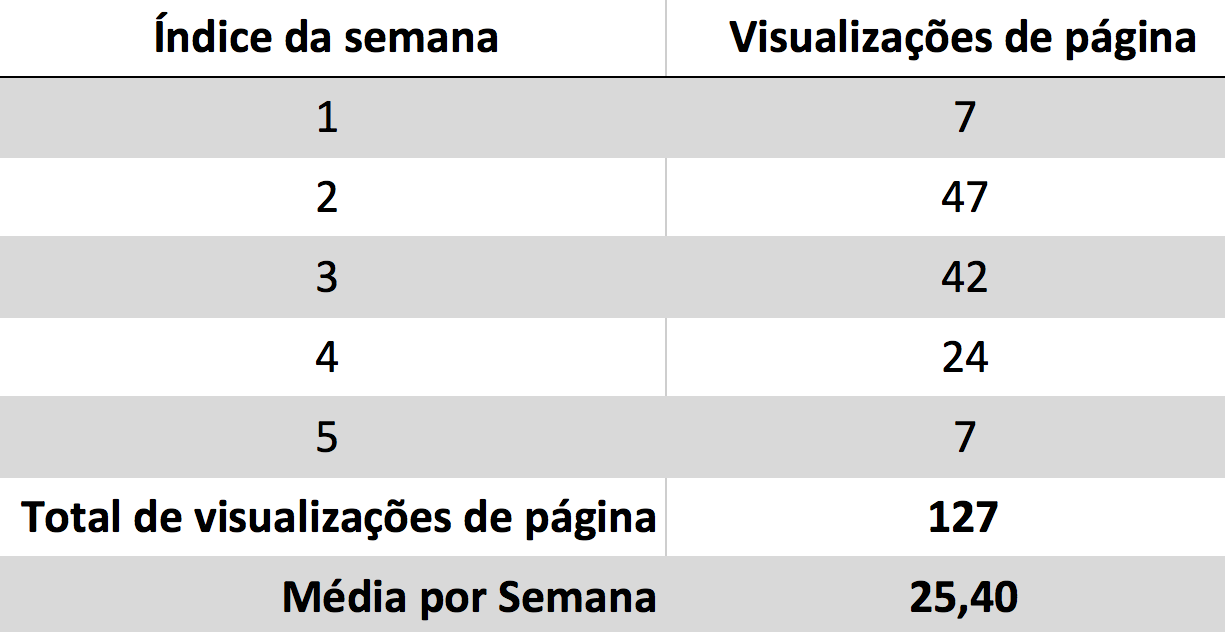
\includegraphics[width=0.6\textwidth]{images/resultados/google-analytics-media-visualizacoes.png}

	\centering
	\footnotesize Fonte: \fonteOAutor
\end{figure}

\FloatBarrier 	% Este comando impede que as imagens
				% flutuem a partir deste ponto no seu documento

Na Figura \ref{fig:googleAnalyticsCidade}, exibe-se as cidades que deram
origem aos acessos à ferramenta de gestão de perguntas e respostas, sendo
que, dentre elas está a cidade de Joinville/SC que é a cidade do autor.

\begin{figure}[h!tb]
	\caption{Cidades em que o acesso ao sistema foi realizado}
	\label{fig:googleAnalyticsCidade}

	\centering
	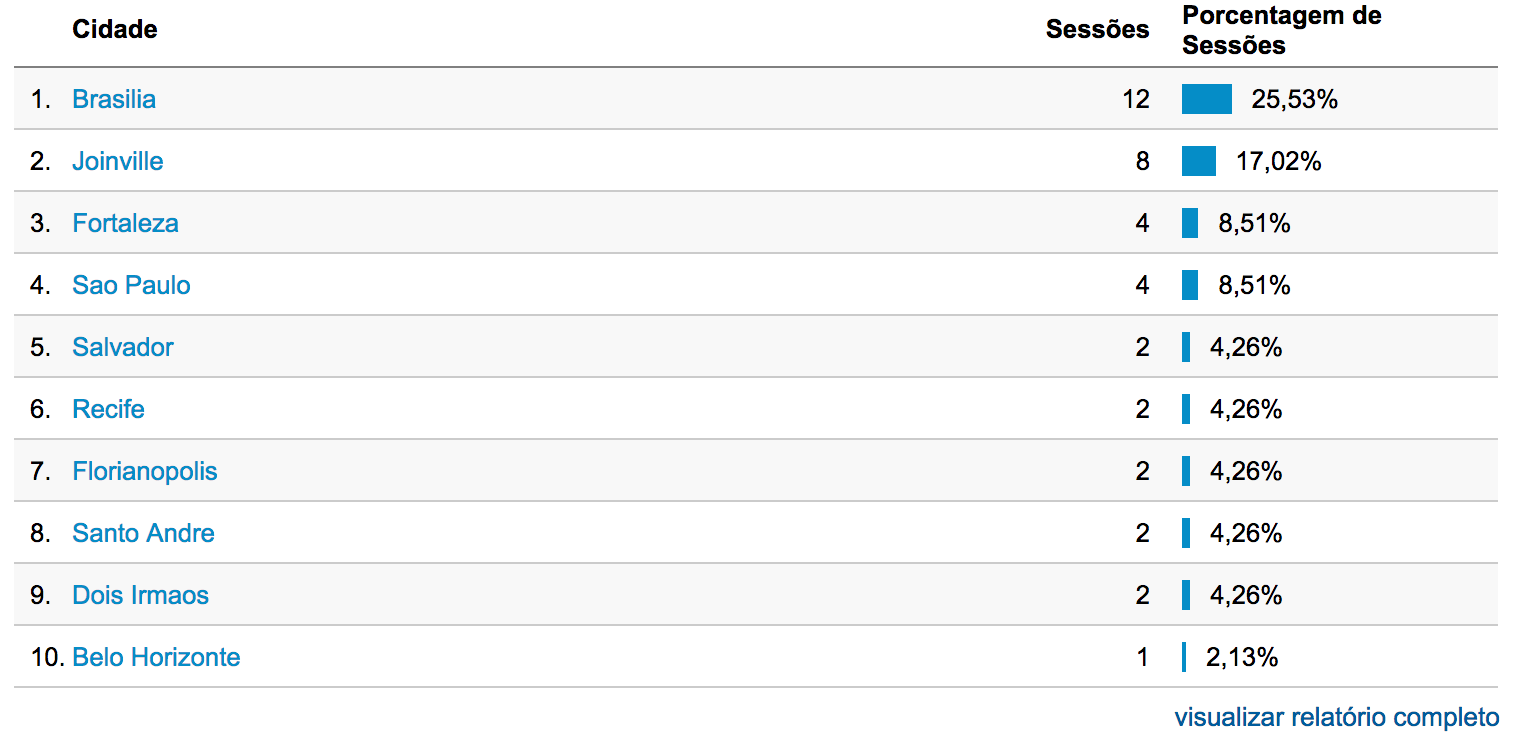
\includegraphics[width=\textwidth]{images/resultados/google-analytics-cidade.png}

	\centering
	\footnotesize Fonte: \fonteOAutor
\end{figure}

\FloatBarrier 	% Este comando impede que as imagens
				% flutuem a partir deste ponto no seu documento
			
Referente a estatísticas de formas de acesso, nenhum uso de \textit{smartphone}
ou \textit{tablet} foi registrado, mas nota-se que dentre os sistemas
operacionais dos profissionais que utilizaram a aplicação está o
\textit{Windows} com 46,81\%, o \textit{Macintosh} com 29,79\% e o
\textit{Linux} com 23,40\%, e em contrapartida, o navegador web mais utilizado 
para o uso da ferramenta foi o \textit{Google Chrome} com 57,45\% do total,
seguido pelo \textit{Firefox} com 38,30\% e pelo \textit{Safari} com 4,26\%
conforme apresenta-se na Figura
\ref{fig:googleAnalyticsSistemaOperacionalNavegador}.

\begin{figure}[h!tb]
	\caption{Sistemas Operacionais e Navegadores utilizados para acesso ao
	sistema web}
	\label{fig:googleAnalyticsSistemaOperacionalNavegador}

	\centering
	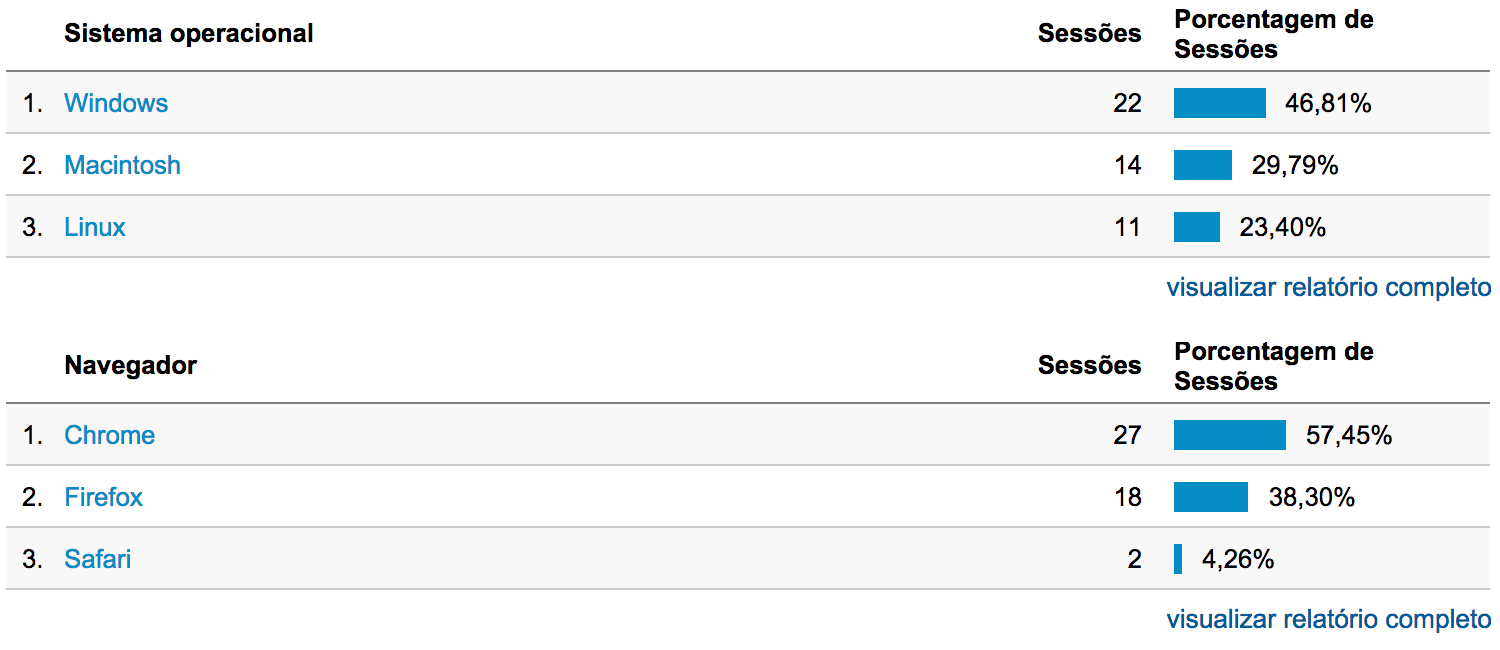
\includegraphics[width=\textwidth]{images/resultados/google-analytics-os-browser.png}

	\centering
	\footnotesize Fonte: \fonteOAutor
\end{figure}

\FloatBarrier 	% Este comando impede que as imagens
				% flutuem a partir deste ponto no seu documento

Nota-se ainda, conforme ilustra a Figura \ref{fig:googleAnalyticsTempoAcesso},
que o tempo médio de acesso à ferramenta é de 02:01 minutos o que permite que um 
colaborador da lista de discussão acesse o sistema gere uma pergunta diária de
maneira anonima e em seguida encerre a sessão, justificando também a taxa de
rejeição de 31,91\%.

\begin{figure}[h!tb]
	\caption{Tempo médio de permanência de um usuário na ferramenta}
	\label{fig:googleAnalyticsTempoAcesso}

	\centering
	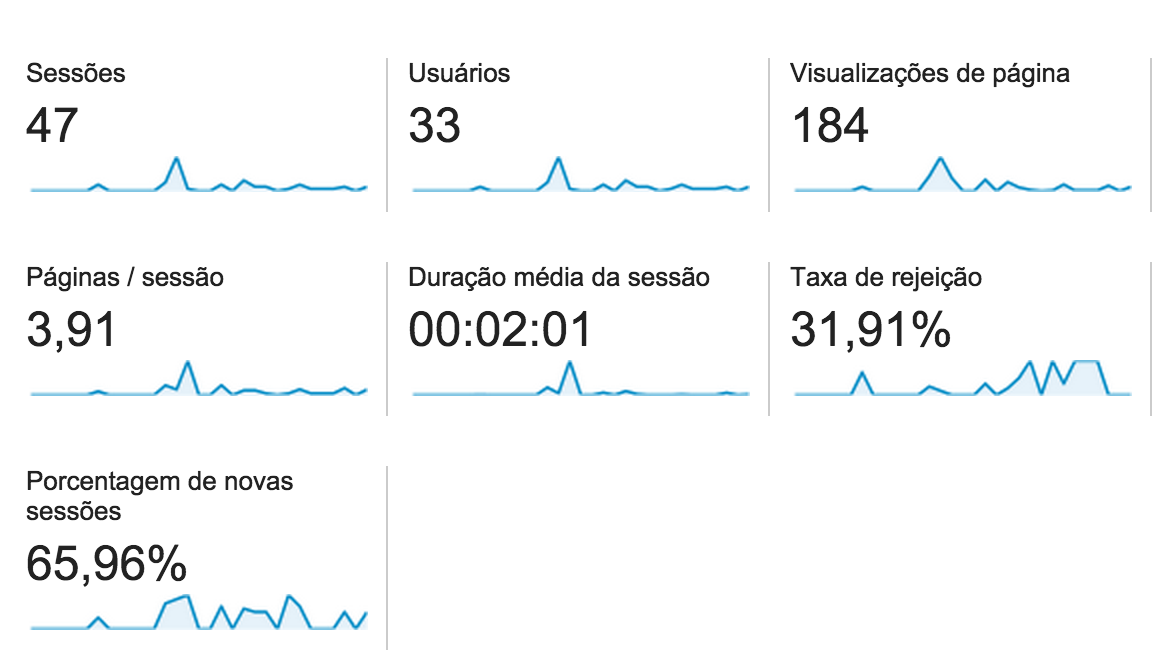
\includegraphics[width=0.7\textwidth]{images/resultados/google-analytics-dados.png}

	\centering
	\footnotesize Fonte: \fonteOAutor
\end{figure}

\FloatBarrier 	% Este comando impede que as imagens
				% flutuem a partir deste ponto no seu documento

Além disto, percebe-se na Figura \ref{fig:googleAnalyticsTempoAcesso} que dentre
as 47 sessões existentes, os 33 usuários navegaram pelo sistema acessando quase
quatro páginas por sessão, outro detalhe importante, é que houve na média mais
do que um acesso por dia ao sistema o que fortalece o fato de que a ferramenta
está sendo utilizada para gerir as perguntas diárias postadas na lista de
discussão.

Na Figura \ref{fig:googleAnalyticsPaginas}, exibe-se as páginas mais acessadas
da aplicação web, nota-se que, todos os usuários entram na página inicial e em
seguida a maioria acessa de forma anonima, entretanto alguns antes de efetuarem
tal ação selecionam um idioma (dentre os disponíveis estão o português do
brasil e o inglês internacional).

\begin{figure}[h!tb]
	\caption{Páginas do sistema mais acessadas}
	\label{fig:googleAnalyticsPaginas}

	\centering
	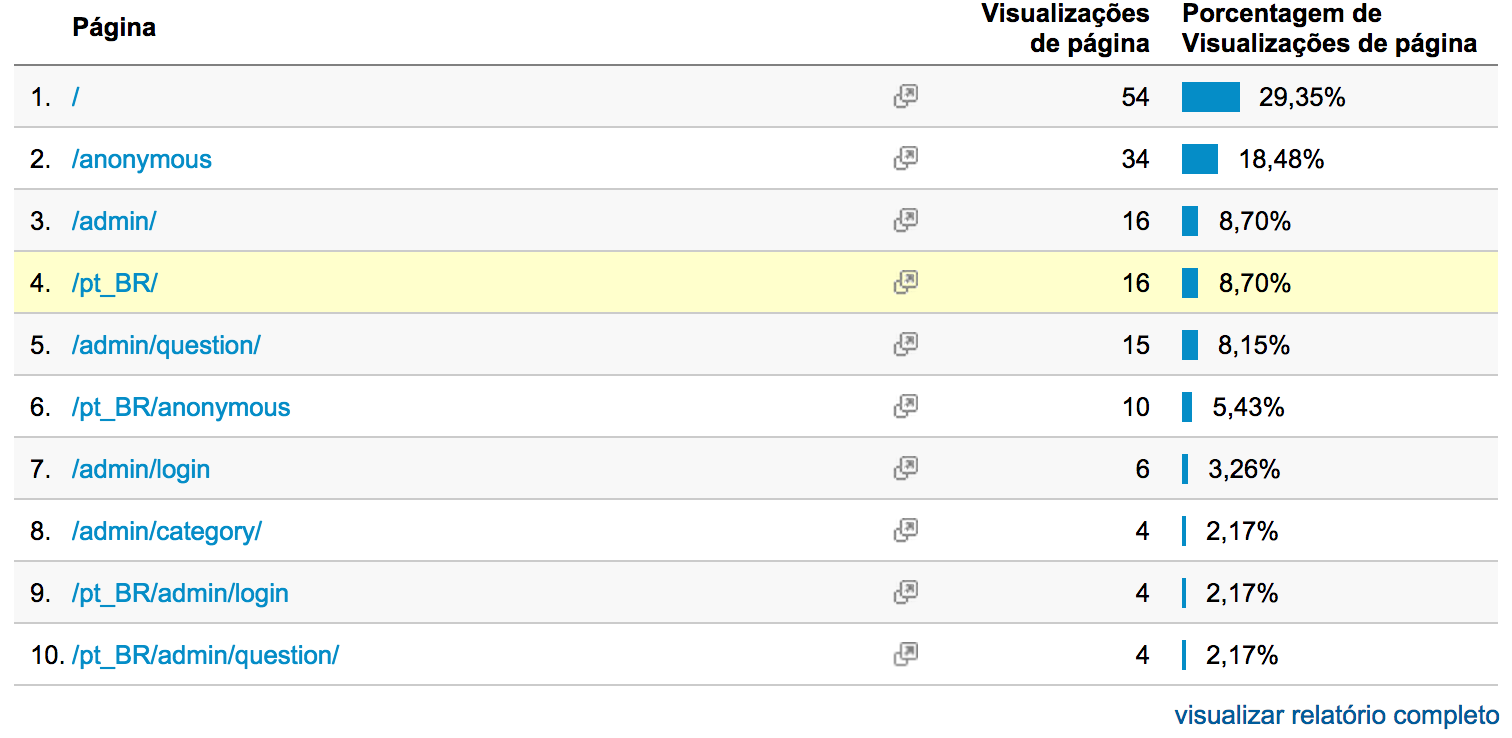
\includegraphics[width=\textwidth]{images/resultados/google-analytics-paginas.png}

	\centering
	\footnotesize Fonte: \fonteOAutor
\end{figure}

\FloatBarrier 	% Este comando impede que as imagens
				% flutuem a partir deste ponto no seu documento

No que diz respeito ao idioma de acesso do sistema, na Figura
\ref{fig:googleAnalyticsIdioma}, exibe-se a quantidade de acessos categorizados
através do idioma dos usuários.

\begin{figure}[h!tb]
	\caption{Idioma dos usuários que realizaram acesso à ferramenta}
	\label{fig:googleAnalyticsIdioma}

	\centering
	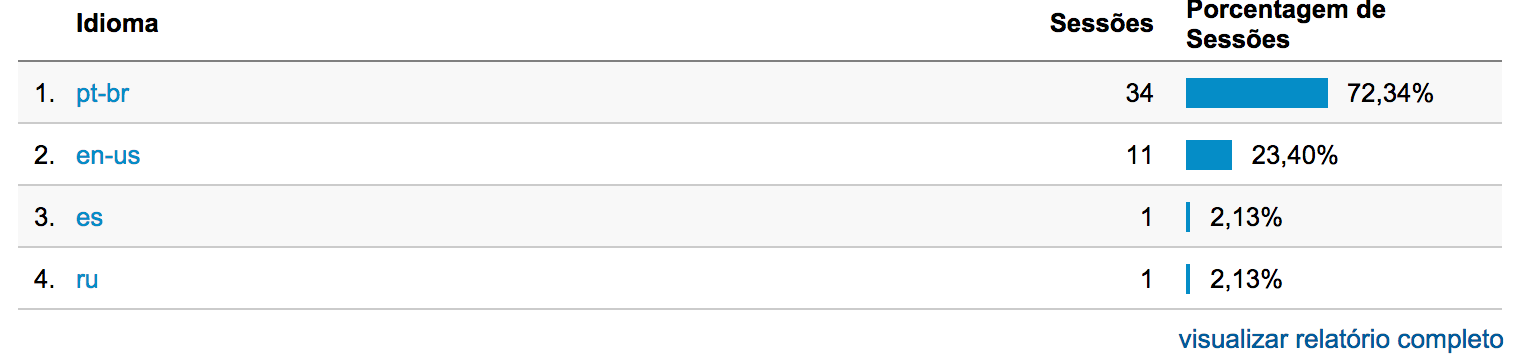
\includegraphics[width=\textwidth]{images/resultados/google-analytics-idioma.png}

	\centering
	\footnotesize Fonte: \fonteOAutor
\end{figure}

\FloatBarrier 	% Este comando impede que as imagens
				% flutuem a partir deste ponto no seu documento

Na Figura \ref{fig:zcpeHome}, exibe-se a página inicial do sistema que apresenta
três maneiras de uso da plataforma, são elas:

\begin{alineas}
    \item anonimamente: permite que o usuário acesse a aplicação sem que haja
    autenticação, liberando acesso para que o usuário gere um template de e-mail
    para disparar manualmente através de seu cliente de e-mail pessoal;
    \item com usuário e senha: permite que o usuário acesse a aplicação com as
    suas credenciais, isto dá direitos para que o usuário gerencie as suas
    próprias perguntas e respostas e dispare e-mails para a lista de discussão
    utilizando uma conta \acs{SMTP} do sistema;
    \item com uma conta google: permite que o usuário realize a autenticação
    através de uma conta \textit{Google}, isto lhe dá as mesmas permissões
    acima, entretanto, o usuário realizará os disparos de e-mail utilizando sua conta
    \textit{Google}.
\end{alineas}

No que se refere aos níveis de acesso  de cada usuário, eles estão organizados
em grupos a fim de facilitar a administração de contas, sendo que, cada grupo
possuí um conjunto de papéis. Além do grupo padrão no qual todos os usuários
da plataforma estão inseridos, há um grupo administrativo que permite gerenciar
as questões que serão exibidas no sistema de simulado e também dá-lhes direito
de gerenciar todas as questões cadastradas no sistema (inclusive as que não são
de sua autoria).

\begin{figure}[h!tb]
	\caption{Página inicial da ferramenta}
	\label{fig:zcpeHome}

	\centering
	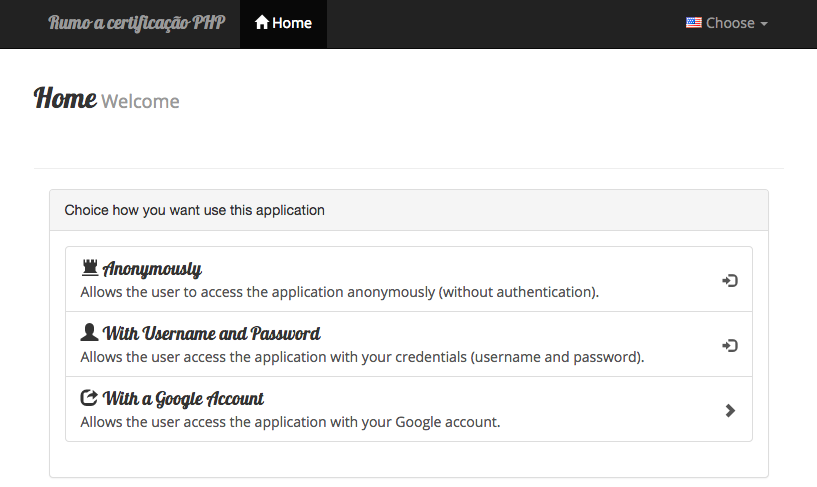
\includegraphics[width=\textwidth]{images/resultados/zcpe-home.png}

	\centering
	\footnotesize Fonte: \fonteOAutor
\end{figure}

\FloatBarrier 	% Este comando impede que as imagens
				% flutuem a partir deste ponto no seu documento

A listagem de perguntas apresentada na Figura \ref{fig:zcpePerguntaListagem}, é
o resultado da categorização de perguntas e respostas da lista de discussão,
sendo que, nesta listagem apresentam-se dados básicos para o usuário que está logado, e para os usuários
administradores exibe-se uma coluna adicional ``aprovado'', sendo que, quando
o valor desta coluna é ``Sim'', então a ferramenta libera a questão
para ser utilizada pelo sistema de simulado.

\begin{figure}[h!tb]
	\caption{Listagem de perguntas}
	\label{fig:zcpePerguntaListagem}

	\centering
	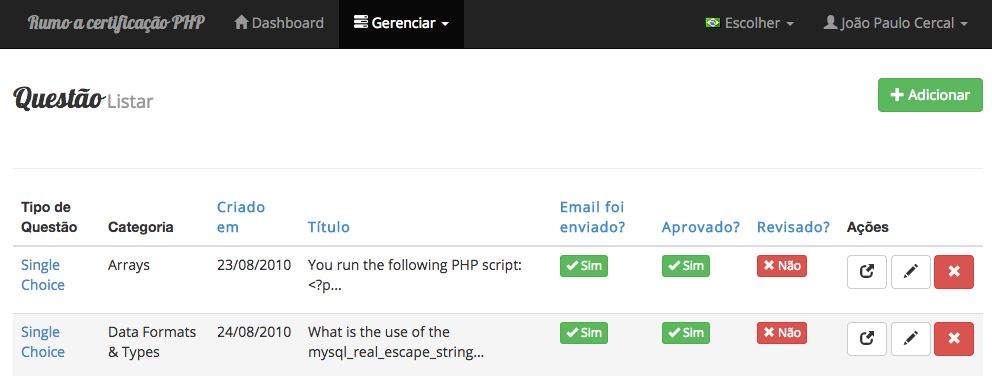
\includegraphics[width=\textwidth]{images/resultados/zcpe-pergunta-listagem.png}

	\centering
	\footnotesize Fonte: \fonteOAutor
\end{figure}

\FloatBarrier 	% Este comando impede que as imagens
				% flutuem a partir deste ponto no seu documento

Na Figura \ref{fig:googleGroupsListagemTopicos}, percebe-se que as questões não
são gerenciadas através de categorias, não há também uma forma de gerenciar as
respostas corretas, outro problema é o fato de que não há somente perguntas na 
listagem de tópicos, por conseguinte a ferramenta proposta eliminou estes
problemas.

\begin{figure}[h!tb]
	\caption{Listagem de tópicos no Google Groups}
	\label{fig:googleGroupsListagemTopicos}

	\centering
	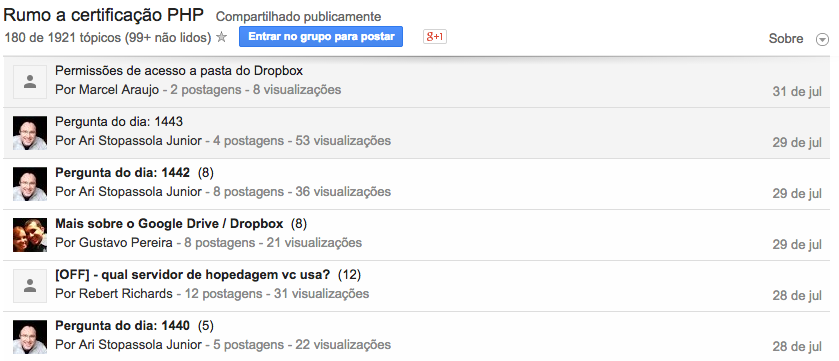
\includegraphics[width=\textwidth]{images/resultados/google-groups-listagem.png}

	\centering
	\footnotesize Fonte: \fonteOAutor
\end{figure}

\FloatBarrier 	% Este comando impede que as imagens
				% flutuem a partir deste ponto no seu documento

Neste momento apresenta-se em detalhes na Figura \ref{fig:zcpePerguntaDetalhes},
a representação da exibição de detalhes de uma questão que está sendo gerenciada
através da ferramenta proposta.

\begin{figure}[h!tb]
	\caption{Detalhes de uma questão}
	\label{fig:zcpePerguntaDetalhes}

	\centering
	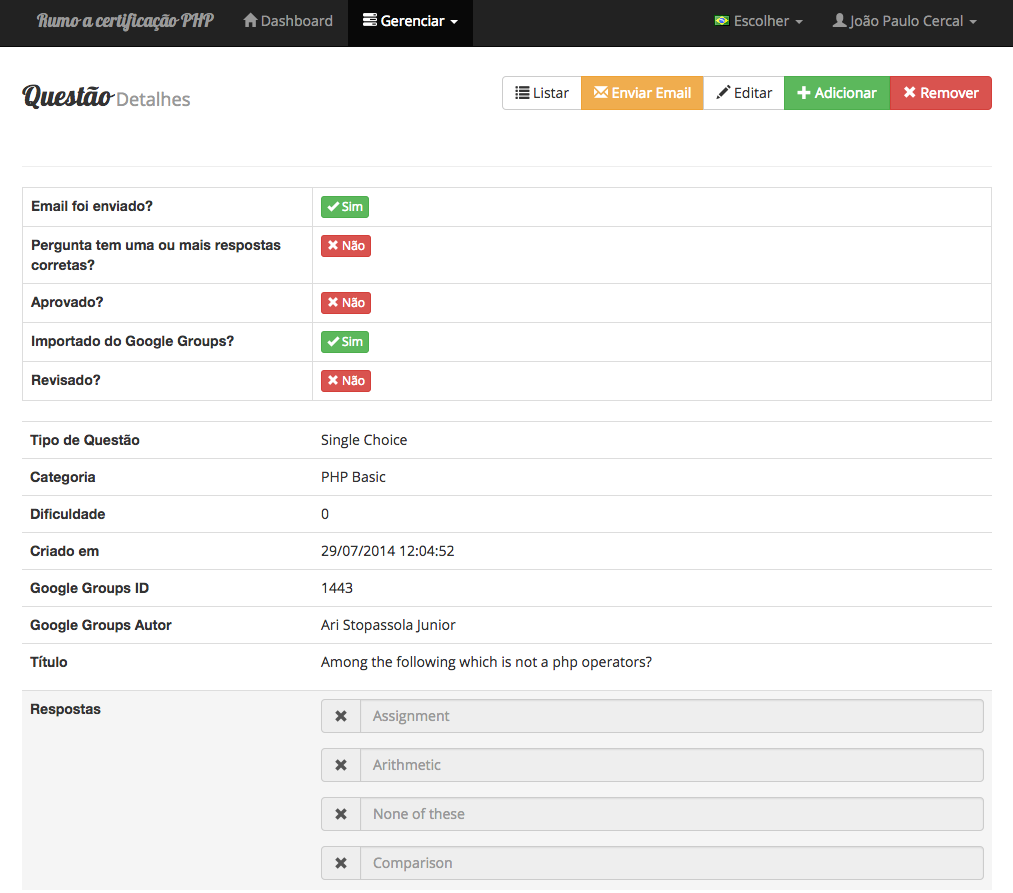
\includegraphics[width=\textwidth]{images/resultados/zcpe-pergunta-detalhes.png}

	\centering
	\footnotesize Fonte: \fonteOAutor
\end{figure}

\FloatBarrier 	% Este comando impede que as imagens
				% flutuem a partir deste ponto no seu documento

Nota-se também que nem todas as informacões que o sistema mantém referente a
questão são exibidos na Figura \ref{fig:zcpePerguntaDetalhes}, sendo que, a
linha ``aprovado'' é exibida apenas para os usuários com permissões
administrativas.

A seguir apresenta-se na Figura \ref{fig:zcpePerguntaDetalhesGoogleGroups}, a
mesma questão na plataforma do \textit{Google Groups} no qual não há nenhum gerenciamento das questões que
foram postadas, diferentemente da nova forma de gestão de perguntas proposta por
este projeto.


\begin{figure}[h!tb]
	\caption{Detalhes da questão 1443 no Google Groups}
	\label{fig:zcpePerguntaDetalhesGoogleGroups}

	\centering
	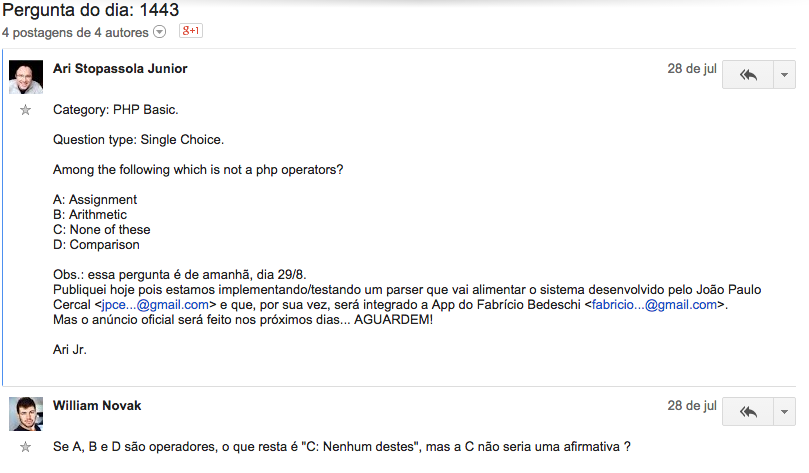
\includegraphics[width=\textwidth]{images/resultados/google-groups-pergunta-1443.png}

	\centering
	\footnotesize Fonte: \fonteOAutor
\end{figure}

\FloatBarrier 	% Este comando impede que as imagens
				% flutuem a partir deste ponto no seu documento
				
Nota-se também que o sistema proposto está internacionalizado e já conta com
dois idiomas, o português do Brasil e o inglês internacional conforme mostra a
Figura \ref{fig:zcpeIdioma}.

\begin{figure}[h!tb]
	\caption{Caixa para seleção do idioma utilizado no sistema}
	\label{fig:zcpeIdioma}

	\centering
	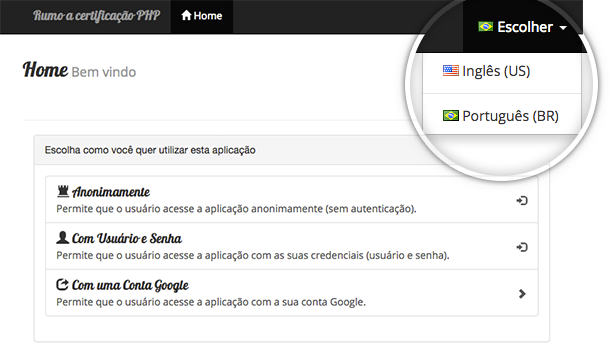
\includegraphics[width=\textwidth]{images/resultados/zcpe-idioma.png}

	\centering
	\footnotesize Fonte: \fonteOAutor
\end{figure}

\FloatBarrier 	% Este comando impede que as imagens
				% flutuem a partir deste ponto no seu documento

Contudo, a proposta deste projeto no que se refere a criação de um ambiente de
simulados não foi concluída, porém, a ferramenta está sendo utilizada para gerir
as perguntas da lista de discussão e pode ser utilizada também para outros fins,
desde que haja semelhança no processo de gerenciamento das questões. A aplicação
web está disponível publicamente no seguinte endereco: \textit{http://zcpe.cekurte.com}.
